\documentclass[10pt]{article}
\usepackage[utf8]{inputenc}
\usepackage{geometry} % to change the page dimensions
\geometry{a4paper}
\usepackage{authblk}

%% Packages
\usepackage{graphicx, subcaption}
\usepackage{amsmath,amssymb,amsthm,amsfonts}
\usepackage{bm}
\usepackage{algorithm, algorithmic}
\usepackage{multirow}
\usepackage{bbm}
\usepackage{kotex}
\usepackage[labelformat=simple]{subcaption}

\usepackage{tikz}
\usetikzlibrary{shapes.geometric, arrows, positioning, calc}
\usetikzlibrary{backgrounds}

\tikzstyle{title} = [rectangle, minimum width=3cm, minimum height=1cm, text centered, draw=black, text width=3cm, fill=white!100]
\tikzstyle{startstop} = [rectangle, rounded corners, minimum width=3cm, minimum height=1cm,text centered, draw=black, fill=red!30]
\tikzstyle{io} = [trapezium, trapezium left angle=70, trapezium right angle=110, minimum width=3cm, minimum height=1cm, text width=1.3cm, text centered, draw=black, fill=blue!30]
\tikzstyle{process} = [rectangle, minimum width=3cm, text width=3cm, minimum height=1cm, text centered, draw=black, fill=orange!30]
\tikzstyle{decision} = [diamond, minimum width=3cm, minimum height=1cm, text centered, draw=black, fill=green!30]
\tikzstyle{arrow} = [thick,->,>=stealth]

\captionsetup[figure]{labelsep=period}
\renewcommand{\thefigure}{\Roman{figure}}
% \captionsetup[subfigure]{labelformat=parens} % default is 'parens'
% \renewcommand{\thesubfigure}{\thefigure.\alph{subfigure}.}
\renewcommand\thesubfigure{(\alph{subfigure})}

%% Theorems
\theoremstyle{plain}
\newtheorem{theorem}{Theorem}[section]
\newtheorem{proposition}[theorem]{Proposition}
\newtheorem{lemma}[theorem]{Lemma}

\theoremstyle{remark}
\newtheorem{remark}[theorem]{Remark}
\newtheorem{example}[theorem]{Example}

\theoremstyle{definition}
\newtheorem{definition}[theorem]{Definition}

%% Equations
\numberwithin{equation}{section}

%% Algorithms
\renewcommand\algorithmicdo{}
\renewcommand\algorithmicthen{}
\renewcommand\algorithmicendfor{\textbf{end}}

%% Macros
\def\chfun{\mathbbm{1}}
\def\skel{\mathcal{S}}
\def\calc{\mathcal{C}}
\def\sko{\hat{\mathcal{S}}}
\def\ske{\mathcal{S}^8}
\def\endske{E\left(\mathcal{S}^8\right)}
\def\endomc{E\left(\Omega_c\right)}


\def\gphi{\nabla\phi}
\def\ngphi{\left|\nabla\phi\right|}
\def\ngphii{\left|\nabla\phi_i\right|}
\def\fci{F_{c,\,i}}
\def\cm{\, ,}
\def\pd{\, .}

\def\omi{\Omega_i}
\def\oma{\Omega_a}
\def\ome{\Omega_E}
\def\omc{\Omega_c}
\def\omcc{\hat{\Omega}_c}

\DeclareMathOperator*{\argmax}{arg\,max}
\DeclareMathOperator*{\argmin}{arg\,min}
% \def\tOmega{\tilde{\Omega}}
% \def\tGamma{\tilde{\Gamma}}
% \def\tV{\tilde{V}}
% \def\W{\mathbb{W}}
% \def\tu{\tilde{u}}
% \def\bu{\bar{u}}
% \def\hu{\hat{u}}
% \def\bl{\bar{\lambda}}
% \def\p{\mathbf{p}}
% \def\P{\mathbf{P}}
% \def\intO{\int_{\Omega}}
% \def\intOs{\int_{\Omega_s}}
% \def\m{\mathbf{m}}
% \def\n{\mathbf{n}}
% \def\blambda{\bm{\lambda}}

% \def\tE{\tilde{E}}
% \def\N{\mathcal{N}}

% \def\div{\mathrm{div}}
% \def\proj{\mathrm{proj}}
% \def\prox{\mathrm{prox}}
% \def\ran{\mathrm{ran}\,}
% \def\ed{\mathrm{ed}}
% \def\supp{\mathrm{supp}\,}
% \def\TOL{\mathrm{TOL}}
% \DeclareMathOperator*{\argmin}{\arg\min}

% Text Color and Strike
\usepackage[normalem]{ulem}
\usepackage{color}
\newcommand{\red}[1]{{\color{red}{#1}}}
\newcommand{\blue}[1]{{\color{blue}{#1}}}

\title{Individual Tooth Segmentation in Two Dimensional Human Teeth Image}
\author{Seongeun Kim}
\affil{Department of Mathematical Sciences, KAIST, Daejeon 34141, Korea}
\date{}

\begin{document}
\maketitle

\begin{abstract}
In this paper, we propose a segmentation method.\end{abstract}

{\small \textbf{Key words}
Image Processing, Neural Networks, Data Processing}

{\small \textbf{AMS subject classifications}
94A08, 68T07}

%% Main text starts ---------------------------------------------------------------------------------------------------
% Section: Introduction
\section{Introduction}
\label{Sec:Introduction}
3차원 치아 복원의 필요성\\
- 전문적인 복원과정의 소모성\\
CT로부터 치아복원 연구들\\
파라노마 이미지로부터 복원 연구들\\
외부에서 촬영된 2차원 치아경계로부터 복원 가능 논문 \cite{WU:2016}\\
연구의 목적

\ref{Subsec:ObtainEr}에서 얻어낸 $\Omega\setminus\omc$의 connected components의 컬렉션을 $\{\omi\}_{i=1}^N$라고 하자. 각각의 연결요소들은 서로소이며, 경계는 그 자체로 active contour를 위한 initial contour가 될 수 있다. 즉, 각 $i$에 대하여, $\partial\Omega_i$를 zero level set으로 갖고, 영역에서 음수인 signed distance function $\phi_{i,\,0}$를 생각할 수 있으며 이 초기 컨투어로부터 정확한 edge를 검출하기 위해 proposed competing force $F_{c,i}$ in a level set formulation:
\begin{align}
    \frac{\partial}{\partial{t}}\phi_i(x,\,t) &= \mu\kappa(\phi_i)\ngphii + \chi_{\Omega\setminus\oma}\fci\ngphii+\chi_{\Omega\setminus\oma}-\chi_{\Omega_a}F_a\cdot \gphi \cm \label{Eq:proposed}\\
    \phi_i(x,\,0) &= \phi_{i,\,0}\,, \nonumber
\end{align}
where $F_a$ is the GADF in \ref{Def:gadf_def}, $F_b$ is the SR force and .

% Sec:Background
\section{Background}
\label{Sec:BG}
In this section, we briefly review geometric attraction-driven flow (GADF) \cite{Hahn:2006, Hahn:2010} and edge region, which plays important role for segmenting individual tooth. We will derive how to obtain edge regions by concerning the problematic features of teeth image.

% Subsec:GADF
\subsection{Geometric Attraction-Driven Flow}
\label{Subsec:GADF}
Assume there is a smooth gray image $I:\Omega\subset\mathbf{R}^2\rightarrow[0,\,1]$. The image intensity changes rapidly on the boundary of two objects in the image. Thus, we define a point $x\in\Omega$ as an edge of the image if
\begin{align}
    % \left.u_x''(s)\right|_{s=0}=0\cm \label{Def:edge}
    u_x''(0)=0\cm \label{Def:edge}
\end{align}
where
\begin{align*}
    u_x(s) = I\left( x + s\frac{\nabla{I(x)}}{|\nabla{I(x)}|} \right)\pd
\end{align*}
The GADF is defined as
\begin{align}
    F_a(x) = \mbox{sgn}(\ell(x))\frac{\nabla I(x)}{\left|\nabla{I(x)}\right|},\quad \forall{x}\in\Omega\cm  \label{Def:gadf}
\end{align}
where the $\mbox{sgn}$ is a sign function and 
\begin{align*}
    \ell(x) &= \int^{\epsilon}_{0} {u'_x(s)} ds - \int^{0}_{-\epsilon} {u'_x(s)} ds\quad\mbox{for a small}~\epsilon > 0\cm
\end{align*}
By the definition, $F_a(x)$ directs the candidates of edges on the line $x + s\frac{\nabla{I(x)}}{|\nabla{I(x)}|}$ that is the points on which $u_x''(s)=0$. An edge region means a region where an edge is thought to exist. In \cite{Hahn:2010}, edge region is defined by using regions where $F_a$ are facing each other, i.e.
\begin{align}
    \Omega_a = \delta_{S_3}\left( \Omega_E \right)\cm \label{Def:edge_region}
\end{align}
where $\delta_{S_3}$ is a dilation function using the $3\times3$ window $S_3$ and 
\begin{align}
    \Omega_E = \left\{ x\in\Omega \mid F_a(x^*) \cdot F_a(x) < 0 ~\mbox{and}~ x^*=x+F_a(x) \right\}\pd \label{Def:pre_er}
\end{align}
Under this setting, contour evolution using a level set formulation that  the initial contour approaches the edge in $\Omega_a$ and goes outward in $\Omega_b = \Omega\setminus \Omega_a$ is proposed:
\begin{align}
    \frac{\partial}{\partial{t}}\phi(x,\,t) &= \alpha\kappa\left|\nabla\phi\right| - \chi_{\oma}F_a\cdot\nabla\phi + \chi_{\Omega_b}F_b|\nabla\phi|\cm \label{Eq:gadf}\\
    \phi(x,\,0) &= \phi_0(x)\cm \nonumber
\end{align}
where $\alpha$ is a constant, $\kappa$ is the curvature of level set functions $\phi$ and $\chi_A$ is a characteristic function on the set $A$.

The GADF is naturally expandable with color images. For a color image $I:\Omega\subset\mathbf{R}^2\rightarrow[0,\,1]^3$, we can consider a nonlinear structure tensor $\mathbf{M}$ from a nonlinear diffusion
\begin{align*}
    \frac{\partial \mathbf{M}(x,\,t)}{\partial t}&=\nabla\cdot\left( h\left( \sum_{i,\,j=1}^2 \left|\nabla M_{ij}(x,\,t)\right|^2  \right) \nabla\mathbf{M}(x,\,t) \right)\cm\\
    \mathbf{M}(x,\,0) &= \sum_{k=1}^3 {\nabla I_k(x)I_k(x)^T}\cm
\end{align*}
and the diffused tensor $\mathbf{M}$ preserves local features of the image $I$ \cite{Rousson:2003, Weickert:2004, Brox:2006, Hahn:2009}. We can count the eigenvector with respect to the maximum eigenvalue of $\mathbf{M}$ as a gradient and then the defining GADF on color images is tractable.

% Subsection: Weak edge detection
\subsection{Weak edge detection}
\label{Subsec:weakedge}
When the change of intensity at the edge of an image is smaller than the neighborhood, we call it a weak edge. For a gray image $I$,
\begin{align*}
    \nabla{|\nabla{I}|} \parallel \mathcal{H}_x(I)\nabla{I}  
\end{align*}
is easily obtained from calculations, and it show that the direction of $\nabla|\nabla{I}|$ is getting differ to the $\nabla{I}$ whenever change of intensities is smaller than neighborhood, because of the affection of the hessian matrix $\mathcal{H}_x(I)$. In other words, around weak edges, it is difficult to determine the edge or edge region simply by using the color information. However, as can be seen in \eqref{Def:gadf}, GADF is defined to have one of the directions of $\nabla{I}$ and $-\nabla{I}$, and thus it is possible to find an edge region that includes all weak edges without regardless of the amount of intensity change. Weak edges are common in human teeth images. In particular, it appears at the boundary between the teeth and the gums and at the boundary between two teeth with similar color and brightness. Figure~\ref{Fig:weak_edges} shows the weak edges seen in the tooth image and the edges or edge regions detected by different methods.

% Figure: Weak edges in teeth image
\begin{figure}
    \centering
    \begin{subfigure}{1\textwidth}
        \centering
        \includegraphics[width=10cm]{./Figures/Fig1_img.png}
        \caption{A whole teeth image}
        \label{fig:1a}
    \end{subfigure} 
    \newline 
    
    \vspace{1mm}

    \begin{subfigure}{.18\textwidth}
        \centering
        \includegraphics[width=2.6cm]{./Figures/Fig1_img1.png}
        \caption{}
    \end{subfigure}
    \begin{subfigure}{.18\textwidth}
        \centering
        \includegraphics[width=2.6cm]{./Figures/Fig1_sbl1.png}
        \caption*{}
    \end{subfigure}
    \begin{subfigure}{.18\textwidth}
        \centering
        \includegraphics[width=2.6cm]{./Figures/Fig1_cny1.png}
        \caption*{}
    \end{subfigure}
    \begin{subfigure}{.18\textwidth}
        \centering
        \includegraphics[width=2.6cm]{./Figures/Fig1_er1.png}
        \caption*{}
    \end{subfigure}\\

    \vspace{1mm}

    \begin{subfigure}{.18\textwidth}
        \centering
        \includegraphics[width=2.6cm]{./Figures/Fig1_img2.png}
        \caption{}
    \end{subfigure}
    \begin{subfigure}{.18\textwidth}
        \centering
        \includegraphics[width=2.6cm]{./Figures/Fig1_sbl2.png}
        \caption*{}
    \end{subfigure}
    \begin{subfigure}{.18\textwidth}
        \centering
        \includegraphics[width=2.6cm]{./Figures/Fig1_cny2.png}
        \caption*{}
    \end{subfigure}
    \begin{subfigure}{.18\textwidth}
        \centering
        \includegraphics[width=2.6cm]{./Figures/Fig1_er2.png}
        \caption*{}
    \end{subfigure}\\

    \vspace{1mm}

    \begin{subfigure}{.18\textwidth}
        \centering
        \includegraphics[width=2.6cm]{./Figures/Fig1_img3.png}
        \caption{}
        \label{Fig:1a3}
    \end{subfigure}
    \begin{subfigure}{.18\textwidth}
        \centering
        \includegraphics[width=2.6cm]{./Figures/Fig1_sbl3.png}
        \caption{}
        \label{Fig:1b3}
    \end{subfigure}
    \begin{subfigure}{.18\textwidth}
        \centering
        \includegraphics[width=2.6cm]{./Figures/Fig1_cny3.png}
        \caption{- 3}
        \label{Fig:1c3}
    \end{subfigure}
    \begin{subfigure}{.18\textwidth}
        \centering
        \includegraphics[width=2.6cm]{./Figures/Fig1_er3.png}
        \caption{- 3}
        \label{Fig:1d3}
    \end{subfigure}
    \caption{(a) A whole teeth image, and sub-images in the red boxes. The results of various methods are shown. (b -- c) Sobel and Canny edge detector with automatically chosen thresholds by MATLAB \cite{MATLAB:R2021a_u1}. (d) $\Omega_E$ from the GADF. }
    \label{Fig:weak_edges}
\end{figure}
    
% Subsection: Edge regions outside the tooth boundaries
\subsection{Edge regions outside the tooth boundaries}
\label{Subsec:eroutside}

In reality, teeth image contains various edges appeared outside of the tooth boundary due to inhomogeneities of the object surface or noise present in the image. Because of these edges, the edge region from GADF includes many connected regions outside the tooth boundary, as shown in Figure~\ref{Fig:1d1}. These unnecessary regions prevent the contours from getting closed to the boundary of interest, so we have to handle them. These regions can be roughly divided into three categories according to the causes:
\begin{itemize}
    \item [(1)] Noise or small stains,
    \item [(2)] Large and faded stains having some clear parts,
    \item [(3)] Strong specular reflections.
\end{itemize} 
(1) The edge regions caused by the tooth boundary are supposed to very large and colors of the image are changed rapidly around them. On the other hand, the edge regions caused by (1) are small and the colors are relatively flat, thus they can be removed by priority \cite{Hahn:2006}. (2) Some stains on the image makes a relatively large edge region. It is not easy to distinguish these regions from edge regions on the tooth boundary only by size and color information. However, if the whole of the stain is not clear and there is some faded parts, then the end of the edge region in that part is exposed. As the initial contour evolves by \ref{Eq:gadf}, if it meets the ends, then it shrinks along the GADF and because of the curvature term, so the edge regions arising from (2) can be canceled out. On the other side, edge regions arises from (3) are in large and closed shape. Because of the shape in which the ends are not exposed, it cannot be handled like (2). These edge regions block the evolution of the contour like a barrier and makes it difficult to find the correct tooth boundary. As a result, they are being main obstacles of the individual tooth segmentation. Contour evolution around the various shaped regions are appeared in Figure~\ref{Fig:er_outside}.

% Figure: Edge regions outside the tooth boundaries
\begin{figure}
    \centering
    % First row
    \begin{subfigure}{.24\textwidth}
        \centering
        \includegraphics[height=2.8cm]{./Figures/Fig2_img.png}
        \caption{}
        \label{Fig:2a}
    \end{subfigure}
    \begin{subfigure}{.24\textwidth}
        \centering
        \includegraphics[height=2.8cm]{./Figures/Fig2_er.png}
        \caption{}
        \label{Fig:2b}
    \end{subfigure}
    \begin{subfigure}{.24\textwidth}
        \centering
        \includegraphics[height=2.8cm]{./Figures/Fig2_reser.png}
        \caption{}
        \label{Fig:2c}
    \end{subfigure}\\
    \vspace{1mm}
    % First row
    \begin{subfigure}{.025\textwidth}
        \centering
        \caption*{\rotatebox[origin=c]{90}{\hspace{-4mm} (d) Left tooth}}
    \end{subfigure}
    \begin{subfigure}{.18\textwidth}
        \centering
        \includegraphics[height=2.4cm]{./Figures/Fig2_evolve_1/iter0.png}
    \end{subfigure}
    \begin{subfigure}{.18\textwidth}
        \centering
        \includegraphics[height=2.4cm]{./Figures/Fig2_evolve_1/iter150.png}
    \end{subfigure}
    \begin{subfigure}{.18\textwidth}
        \centering
        \includegraphics[height=2.4cm]{./Figures/Fig2_evolve_1/iter250.png}
    \end{subfigure}
    \begin{subfigure}{.18\textwidth}
        \centering
        \includegraphics[height=2.4cm]{./Figures/Fig2_evolve_1/iter300.png}
    \end{subfigure}
    \begin{subfigure}{.18\textwidth}
        \centering
        \includegraphics[height=2.4cm]{./Figures/Fig2_evolve_1/iter1000.png}
    \end{subfigure}\\
    \vspace{1mm}
    % Second row
    \begin{subfigure}{.025\textwidth}
        \centering
        \caption*{\rotatebox[origin=c]{90}{\hspace{-4mm} (e) Right tooth}}
    \end{subfigure}
    \begin{subfigure}{.18\textwidth}
        \centering
        \includegraphics[height=2.4cm]{./Figures/Fig2_evolve_2/iter0.png}
    \end{subfigure}
    \begin{subfigure}{.18\textwidth}
        \centering
        \includegraphics[height=2.4cm]{./Figures/Fig2_evolve_2/iter200.png}
    \end{subfigure}
    \begin{subfigure}{.18\textwidth}
        \centering
        \includegraphics[height=2.4cm]{./Figures/Fig2_evolve_2/iter350.png}
    \end{subfigure}
    \begin{subfigure}{.18\textwidth}
        \centering
        \includegraphics[height=2.4cm]{./Figures/Fig2_evolve_2/iter650.png}
    \end{subfigure}
    \begin{subfigure}{.18\textwidth}
        \centering
        \includegraphics[height=2.4cm]{./Figures/Fig2_evolve_2/iter1000.png}
    \end{subfigure}\\
    \vspace{1mm}
    % Third row
    \begin{subfigure}{.025\textwidth}
        \caption*{\rotatebox[origin=c]{90}{\hspace{-3mm} (f) Outside}}
    \end{subfigure}
    \begin{subfigure}{.18\textwidth}
        \centering
        \includegraphics[height=2.4cm]{./Figures/Fig2_evolve_3/iter0.png}
    \end{subfigure}
    \begin{subfigure}{.18\textwidth}
        \centering
        \includegraphics[height=2.4cm]{./Figures/Fig2_evolve_3/iter200.png}
    \end{subfigure}
    \begin{subfigure}{.18\textwidth}
        \centering
        \includegraphics[height=2.4cm]{./Figures/Fig2_evolve_3/iter350.png}
    \end{subfigure}
    \begin{subfigure}{.18\textwidth}
        \centering
        \includegraphics[height=2.4cm]{./Figures/Fig2_evolve_3/iter650.png}
    \end{subfigure}
    \begin{subfigure}{.18\textwidth}
        \centering
        \includegraphics[height=2.4cm]{./Figures/Fig2_evolve_3/iter1000.png}
    \end{subfigure}\\

    \caption{(a) Teeth image in which with presence of light reflections. (b) The region $\Omega_E$ of (a). (c) Result obtained by removing regions caused by (a) in the Section~\ref{Subsec:eroutside} and dilated. (d -- f) From left to right, the contour evolution process over time is shown. The leftmost part is the initial contour state, and the rightmost part is when the steady state is reached. From left to right, contour evolving process are appeared with initial contours located at (d) left tooth, (e) right tooth and (f) outside of teeth. Observe that the contour pushes into exposal ends in (c) but cannot cross the massive, closed regions and stops. Especially in (d), contour even cannot reach whole part of tooth boundary.}
    \label{Fig:er_outside}
\end{figure}

% Subsection: Avoidance of light reflections in the teeth image
\subsection{Avoidance of light reflections in the teeth image}
\label{Subsec:avoidance}

There are previous studies that try to remove light reflections on a single image \cite{SpecRemoval:2006,SpecRemoval:2015,SpecRemoval:2016,SpecRemoval:2018}. They attempts to separate an image with reflections into an image without reflections and reflections and for this, image intensity histogram is used or a dichromatic image model is assumed. This methods are based on color information of the reflective region but in the case of teeth images, due to the nature of the human teeth, the light reflection and the color of the tooth surface are almost the same. For this reason, when the existing methods are actually applied, a part of the tooth surface is also removed with light reflection. 

There have also been attempts to remove light reflection on teeth images by using the single layer perceptron \cite{LeeRemoval:2010}, but it has a limitation that it cannot be applied to a wide range, because learning is processed using only one image as well as the perceptron has an extremely simple structure.

Above all, even if light reflection is removed from the teeth image, individual tooth cannot be segmented immediately. If a lot of unnecessary edges appear due to stains or noise, it is still difficult to separate individual teeth. In addition, if light reflection appears on the tooth boundary, the edge itself would collapse when the light reflection is removed, and making it impossible to detect. Therefore, we seek a method to directly obtain only the edge region near the tooth boundary regardless of any stains, noise or reflections of the image, and for this, a supervised learning method for deep neural networks is considered.

% Section: Proposed Method
\section{Proposed Method}
\label{Sec:PM}
In this section, we describe the steps of the proposed individual tooth segmentation. It is done through the following three main steps, and the whole process is shown in the Figure~\ref{Fig:flowchart}:

\begin{itemize}
    \item[(1)] Data labeling and training strategy,
    \item[(2)] Obtaining an edge region candidate from a neural network and region trimming,
    \item[(3)] Segmentation using active contours competing with each other,
    \item[(4)] Teeth and non-teeth region classification.
\end{itemize}

% Figure: Algorithm flowchart
\begin{figure}
    \centering
    \begin{subfigure}[]{1\textwidth}
        % \centering
        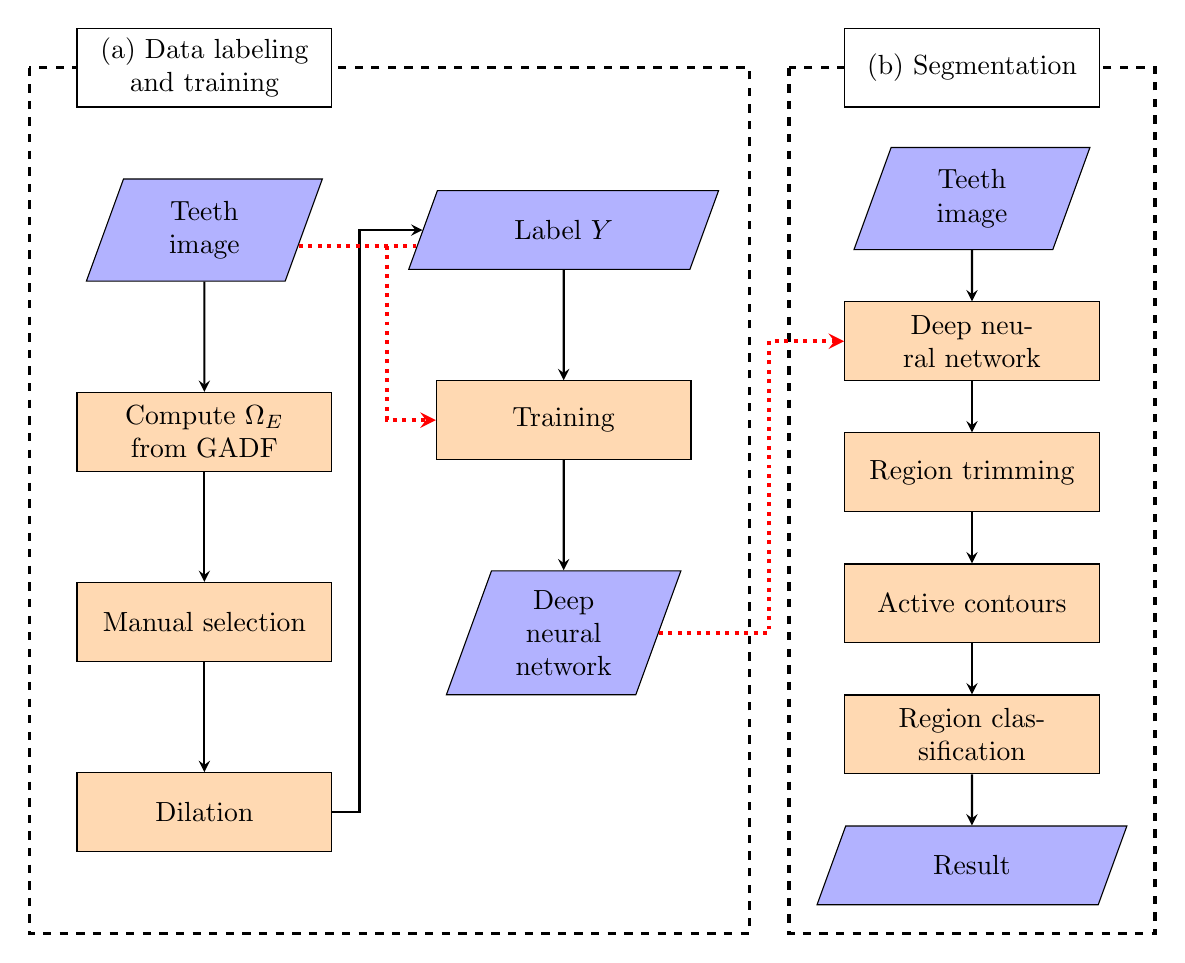
\begin{tikzpicture}[node distance=1.4cm and 1.5cm]
            \node (title1) [title] {(a) Data labeling and training};
            \node (title3) [title, right=6.5cm of title1] {(b) Segmentation};
            \node (teeth1) [io, below=.9cm of title1] {Teeth image};
            \node (pro11) [process, below=of teeth1] {Compute $\Omega_E$ from GADF};
            \node (pro12) [process, below=of pro11] {Manual selection};
            \node (pro13) [process, below=of pro12] {Dilation};
            \node (label) [io, right=of teeth1] {Label $Y$};
            \node (pro14) [process, below=of label] {Training};
            \node (dnn) [io, below=of pro14] {Deep neural network};
            
            \node (teeth3) [io, below=.5cm of title3] {Teeth image};
            \node (pro31) [process, below=.65cm of teeth3] {Deep neural network};
            \node (pro32) [process, below=.65cm of pro31] {Region trimming};
            \node (pro33) [process, below=.65cm of pro32] {Active contours};
            \node (pro34) [process, below=.65cm of pro33] {Region classification};
            \node (res) [io, below=.65cm of pro34] {Result};
            
            \draw [arrow] (teeth1) -- (pro11);
            \draw [arrow] (pro11) -- (pro12);
            \draw [arrow] (pro12) -- (pro13);
            \draw [arrow] (pro13.east) -| ($(label.west) + (-.8, 0)$) -- (label.west);
            \draw [arrow] (label) -- (pro14);
            \draw [arrow] (pro14) -- (dnn);
            \draw [arrow] (teeth3) -- (pro31);
            \draw [arrow] (pro31) -- (pro32);
            \draw [arrow] (pro32) -- (pro33);
            \draw [arrow] (pro33) -- (pro34);
            \draw [arrow] (pro34) -- (res);

            \draw [red,line width=.5mm,dotted] ($(teeth1.east) + (-.07, -.2)$) |- ($(label.west) + (-.07, -.2)$);
            \draw [arrow, red,line width=.5mm, dotted] ($(label.west) + (-.45, -.2)$) |- (pro14.west);
            \draw [arrow, red,line width=.5mm, dotted] (dnn.east) -| ($(pro31.west) + (-.95,0)$) -- (pro31.west);
            \begin{scope}[on background layer]
                \draw[black,line width=.4mm,dashed] ($(title1.west)+(-.6,0)$)  rectangle ($(title1.east)+(5.3,-11)$);
                \draw[black,line width=.4mm,dashed] ($(title3.west)+(-.7,0)$)  rectangle ($(title3.east)+(.7,-11)$);
            \end{scope}
        \end{tikzpicture}
    \end{subfigure}
    \caption{Algorithm flowchart of (a) the labeling and training and (b) segmentation process.}
    \label{Fig:flowchart}
\end{figure}
    
% Subsection: Data labeling and training strategy
\subsection{Data labeling and training strategy}
\label{Subsec:DLT}

Labels for input data are indispensable for supervised learning. In general, labels do not accompany the data, and they should be create them by human force. However, human labeling has to pay too much time and effort, and also has a big disadvantage that there is no guarantee that the label completely matches the information of the image. For example, we want to take the edge region on tooth boundary as label, and the $\Omega_E$ obtained from GADF are on the point that exactly satisfies \ref{Def:edge}, whereas there is no such assurance in the case of direct labeling by humans. Therefore, we devise a labeling method that reflects the information of the teeth image well while minimizing the human touch. In the left of Figure~\ref{Fig:flowchart}, algorithm flowchart of the labeling and training process are displayed. First, compute the region $\Omega_E$ where GADF faces each other and manually select connected components of $\Omega_E$ only present on the tooth boundary, let's denotes the selected region $\Omega_S$. After that, the label $Y:\Omega\subset\mathbf{R}^2\rightarrow\{0,\,1\}$ is obtained as
\begin{align*}
    Y(x) =
    \begin{cases}
        1 & \mbox{in}~\delta_{S_\omega}(\Omega_S)\cm\\
        0 & \mbox{otherwise}
    \end{cases}
\end{align*}
by the dilation $\delta_{S_\omega}$. This process can be viewed in the Figure~\ref{Fig:labeling}.

In the labeling, we did only selection process to minimize human touch. Because of this simplicity, the label does not perfectly match the tooth boundaries. For example, the label contains unnecessary parts which are actually not related to the tooth boundary but selected because they are connected to them. And also many leakages are occurs. See Figure~\ref{Fig:4d}. 

% Figure: Experimental results
\begin{figure}[]
    \centering
    \begin{subfigure}[]{.4\textwidth}
        \centering
        \includegraphics[height=3.8cm]{./Figures/Fig4_img.pdf}
        \caption{}
        \label{Fig:4a}
    \end{subfigure}
    \begin{subfigure}[]{.4\textwidth}
        \centering
        \includegraphics[height=3.8cm]{./Figures/Fig4_er.pdf}
        \caption{}
        \label{Fig:4b}
    \end{subfigure}\\
    \vspace{1mm}
    \begin{subfigure}[]{.4\textwidth}
        \centering
        \includegraphics[height=3.8cm]{./Figures/Fig4_seler.pdf}
        \caption{}
        \label{Fig:4c}
    \end{subfigure}
    \begin{subfigure}[]{.4\textwidth}
        \centering
        \includegraphics[height=3.8cm]{./Figures/Fig4_label.pdf}
        \caption{}
        \label{Fig:4d}
    \end{subfigure}
    \caption{Algorithm flowchart of the labeling process}
    \label{Fig:labeling}
\end{figure}

In general, the labels used for training are considered fit perfectly to the data. Therefore, well-known image-to-image networks \cite{Ronneberger:2015, Wang:2020} have connections to preserve features at high resolution, in order to keep even the smallest details of a label. However, since the details in the labels are corrupted in our case, we can predict that the result will also have corrupted details if we try to train to retain all the details in the label. Therefore, to avoid not only the regions outside tooth boundary but also corrupted details in the labels, we use an encoder-decoder model having a latent space with much smaller dimension compared to the input. The structure of the neural network that we use is appeared in Figure~\ref{Fig:network}.

% Figure: Network structure
\begin{figure}[]
    \centering
    \subfloat[][]{ \includegraphics[height=4.8cm]{./Figures/Fig1_img.png} }
    \caption{Network structure}
    \label{Fig:network}
\end{figure}

% Subsection: Obtaining an edge region candidate from a neural network and region trimming
\subsection{Obtaining an edge region candidate of from a neural network and region trimming}
\label{Subsec:ObtainEr}

The neural network obtained from the Section~\ref{Subsec:DLT} infers a probability map $\hat{Y}:\Omega\in\mathbf{R}^2\rightarrow\left[0,\,1\right]$ when it takes an image $I:\Omega\rightarrow\left[0,\,1\right]$. Here $\hat{Y}(x)$ is the probability of having an edge on tooth boundary at $x$. We call the region defined by
\begin{align*}
    \omc = \left\{ x\in\Omega \mid \hat{Y}(x) > \alpha \right\}
\end{align*}
as an edge region candidate $I$ from the neural network and it is shown in (b) of Figure~\ref{Fig:er_cand}.
% Figure: Edge region candidate
\begin{figure}[]
    \centering
    \begin{subfigure}[]{.4\textwidth}
        \centering
        \includegraphics[width=5.8cm]{./Figures/Fig6_img0.pdf}
        \includegraphics[width=5.8cm]{./Figures/Fig6_img1.pdf}
        \includegraphics[width=5.8cm]{./Figures/Fig6_img8.pdf}
        \includegraphics[width=5.8cm]{./Figures/Fig6_img17.pdf}
        \caption{Input images}
    \end{subfigure}
    \begin{subfigure}[]{.4\textwidth}
        \centering
        \includegraphics[width=5.8cm]{./Figures/Fig6_neter0.pdf}
        \includegraphics[width=5.8cm]{./Figures/Fig6_neter1.pdf}
        \includegraphics[width=5.8cm]{./Figures/Fig6_neter8.pdf}
        \includegraphics[width=5.8cm]{./Figures/Fig6_neter17.pdf}
        \caption{Edge region candidates $\omc$}
    \end{subfigure}
    \caption{Input images and obtained edge region candidates $\omc$. }
    \label{Fig:er_cand}
\end{figure}
One notable point is that the majority of $\omc$ are correctly located on the tooth boundary, although the label included many unnecessary regions. 

On the other hand, $\omc$ is not yet perfect. It contains small fragments and leakages, and thus we apply a trimming process to $\omc$ by forming closed individual tooth regions. First, small fragments and holes can be easily removed and filled in compared to the size of $\Omega$. To deal with the leakages, it is required that figuring out where the leakages occurs. We assume that the leakages are always exist with ends of $\omc$ and thus, we can fill the leakages by finding the ends and extending them. Since $\omc$ is a region obtained by thresholding the probability map, the thickness and shape of the region are not uniform, and so it is not easy to mathematically define the end. Furthermore, in order to decide which direction to extend the region at the end, the direction in which the region travels must be obtained, but it is not easy to find the direction directly from $\omc$. By investigating to the concepts of topological skeletons \cite{Blum:1967} and 8-pixel connectivities \cite{Jonker:1992}, we were able to define ends and representative parametric curve for $\omc$. In the Figure~\ref{Fig:ex_ends}, it shows the ends and the curves obtained from the 8-connected skeleton. 

\subsubsection{Finding edges and extension from the edge}
\label{Ssubsec:skeleton}
The topological skeleton of $\omc$ can be defined in various ways that are equivalent to each other. In this paper, we use the ridge of a signed distance function:
\begin{align*}
    \skel = \left\{ x\in \omc \mid |\nabla\phi(x)| = 0 \right\}\cm
\end{align*}
where $\phi = \mbox{SDF}(\omc)$. This can be discretized in a natural way, and let the notation $\sko$ denote the discretized version. By assuming the pixel connectivities, there may exist distinct subsets of $\sko$ whose 8-connectivities are coincide. In this manner, two sets $A\subset B$ are defined to be related if
\begin{align*}
    \forall R\subset\mathcal{R}_A,\quad\exists! R'\subset\mathcal{R}_B\quad\mbox{such that}\quad C\subset D\cm
\end{align*}
and denoted as $A\sim B$. Here, $\mathcal{R}_A^8,\,\mathcal{R}_B^8$ are the set of all 8-connected components of $A$ and $B$, respectively.
Now consider a set $\calc$ defined as
\begin{align*}
    \calc = \left\{ C\sim\sko \mid \forall x\in C,\quad C\setminus\{x\} \nsim \sko \right\}\cm
\end{align*}
and let $\ske\in\calc$ be a maximal element. We call the $\ske$ as an 8-connected skelton of $\omc$. Observe that $\calc$ is a partially ordered set and so $\ske$ does not need to unique, but the existence of $\ske$ is obvious because of the trivial element of $\calc$. Look at the Figure~\ref{Fig:ends}, we define a point $x$ of a skeleton as an end if $S_3(x)$ is the same as one of the figures and let the set of all such ends be $\endske$. As seen in the figures, there are only two points, the end point itself and the other point when $x\in\endske$. Let the end point be $x_0$ and let the other point be $x_1$. If $x_1\notin\endske$, there may be several points other than $x_0$ and $x_1$ in $S_3(x_1)$. Choose $x_2\in S_3(x_1)$, the next point, to be the farthest point from $x_0$, the previous point, among the other points. By doing this repeatedly, we can obtain a parametric curve $\gamma_e:\mathbf{Z}\cap[0,\,L]\rightarrow\Omega$ given by
\begin{align*}
    \gamma_e(n) = x_n,\quad n=0,\,1,\,\cdots,\,L\cm
\end{align*}
where $e\in\endske$ and $L$ is a positive integer.

% Figure: ends of 8-conn
\newcommand*{\gsz}{.8}%
\newcommand*{\xgap}{3.2}%
\newcommand*{\ygap}{3.2}%
\begin{figure}[]
    \centering
    \begin{tikzpicture}
        \foreach \i in {0,...,3} {
            \foreach \j in {0, 1} {
                \draw [step=\gsz, black, thick, fill=black!20!white] (-\gsz * 5 + \i * \xgap, \j * \ygap) grid ($(-\gsz * 5 + \i * \xgap, \j * \ygap) + (\gsz * 3, \gsz * 3)$) rectangle (-\gsz * 5 + \i * \xgap, \j * \ygap);
                \draw [black, thick, fill=yellow!45!white] ($(-\gsz * 5 + \i * \xgap, \j * \ygap) + (\gsz, \gsz)$) rectangle ($(-\gsz * 5 + \i * \xgap, \j * \ygap) + (\gsz * 2, \gsz * 2)$);
            }
        }
        \draw [black, thick, fill=yellow!45!white] (-\gsz * 5 + 0 * \xgap, 0 * \ygap) rectangle ++(\gsz, \gsz);
        \draw [black, thick, fill=yellow!45!white] (-\gsz * 5 + 1 * \xgap + \gsz, 0 * \ygap) rectangle ++(\gsz, \gsz);
        \draw [black, thick, fill=yellow!45!white] (-\gsz * 5 + 2 * \xgap + 2 * \gsz, 0 * \ygap) rectangle ++(\gsz, \gsz);
        \draw [black, thick, fill=yellow!45!white] (-\gsz * 5 + 3 * \xgap + 2 * \gsz, 0 * \ygap + \gsz) rectangle ++(\gsz, \gsz);
        \draw [black, thick, fill=yellow!45!white] (-\gsz * 5 + 3 * \xgap + 2 * \gsz, 1 * \ygap + 2 * \gsz) rectangle ++(\gsz, \gsz);
        \draw [black, thick, fill=yellow!45!white] (-\gsz * 5 + 3 * \xgap + 2 * \gsz, 1 * \ygap + 2 * \gsz) rectangle ++(\gsz, \gsz);
        \draw [black, thick, fill=yellow!45!white] (-\gsz * 5 + 3 * \xgap + 2 * \gsz, 1 * \ygap + 2 * \gsz) rectangle ++(\gsz, \gsz);
        \draw [black, thick, fill=yellow!45!white] (-\gsz * 5 + 2 * \xgap + 1 * \gsz, 1 * \ygap + 2 * \gsz) rectangle ++(\gsz, \gsz);
        \draw [black, thick, fill=yellow!45!white] (-\gsz * 5 + 1 * \xgap + 0 * \gsz, 1 * \ygap + 2 * \gsz) rectangle ++(\gsz, \gsz);
        \draw [black, thick, fill=yellow!45!white] (-\gsz * 5 + 0 * \xgap + 0 * \gsz, 1 * \ygap + 1 * \gsz) rectangle ++(\gsz, \gsz);
    \end{tikzpicture}
    \caption{The eight situations with ends of skeleton and their neighbors. The points in the skeleton are highlighted in yellow.}
    \label{Fig:ends}
\end{figure}

\subsubsection{Extension from ends}
\label{Ssubsec:extend}

Now the ends and directions on the set $\omc$ are defined using the $\endske$ and $\gamma_e(t)$. The end of $\omc$ is defined by assuming that $\omc$ is cut by normal line at the $\gamma_e(L)$. The connected part of $\omc$ which contains $e$ is considered as an end of $\omc$. We can calculate tangents and curvatures of $\gamma_e$ for every $e\in\endske$ and from now, we regard the tangents and curvatures as at the end of $\ske$. We plan to fill the leakages by trying to extend it by sequentially seeking more plausible direction. The basic strategy in this process is returning to the end after a bad extension, that is, if the leakage is not closed after a certain length of extension, then return to the end and start extension in the next direction. This is because we do not want to complicate the region by extensions that cannot reached, and it is assume that if the direction is appropriate, then the ends should be able to fill the leakages with even a not very long extension. There are three different cases:
\begin{itemize}
    \item [(1)] Using $\ome$ coincident with the direction of the end.\\
    Suppose that $\omc$ continued along an edge of an image and breaks. If the edge is still continued even in the resulted leakage, then $\ome$ should exist with the same direction as $\omc$. Therefore, we extend the end along $\ome$ when the directions of $\ome$ and $\omc$ are similar at the end, i.e.,
    \begin{align*}
        |T(e) \cdot F_a(e)| < \frac{1}{2},\quad e\in E(\ske).
    \end{align*}

    \item [(2)] Using quadratic curve.\\
    When there are no $\ome$ with the same direction at the end, then we extend the end following the quadratic curve which is the best quadratic approximation of the all points of the end of $\omc$, in a least square sense.

    \item [(3)] Using straight line.\\
    The remaining leakages can be filled with an extension along the best linear approximation in a least square sense.
\end{itemize}
We call the resulting region obtained from $\omc$ as $\omcc$. In the Figure~\ref{Fig:ex_ends_d}, the ends, curves and extended result are appeared.

% Figure: skeleton
\begin{figure}[]
    \centering
    \begin{subfigure}[]{.24\textwidth}
        \centering
        \includegraphics[height=3.5cm]{./Figures/Fig8_img.pdf}
        \caption{}
        \label{Fig:ex_ends_a}
    \end{subfigure}
    \begin{subfigure}[]{.24\textwidth}
        \centering
        \includegraphics[height=3.5cm]{./Figures/Fig8_curve.pdf}
        \caption{}
        \label{Fig:ex_ends_b}
    \end{subfigure}
    \vspace{1mm}
    \begin{subfigure}[]{.24\textwidth}
        \centering
        \includegraphics[height=3.5cm]{./Figures/Fig8_end.pdf}
        \caption{}
        \label{Fig:ex_ends_c}
    \end{subfigure}
    \begin{subfigure}[]{.24\textwidth}
        \centering
        \includegraphics[height=3.5cm]{./Figures/Fig8_ext.pdf}
        \caption{}
        \label{Fig:ex_ends_d}
    \end{subfigure}
    \caption{The process of finding ends and extension from the ends are appeared. (b) The parametric curve $\gamma_e$ for all $e\in\endske$ are presented on $\omc$ of the teeth image (a). The ends are highlighted using blue dots. (c) The ends of $\omc$ are highlighted in red color and (d) extension result $\omcc$.}
    \label{Fig:ex_ends}
\end{figure}

% Subsection: Segmentation using balloon shaped competing force
\subsection{Segmentation using balloon shaped competing force}
\label{Subsec:SegLevelset}

Let $\{\Omega_i\}_{i=1}^N$ be a collection of disjoint subsets of a given domain $\Omega\subset\mathbf{R}^2$ such that
\begin{align*}
    \bigcup_{i=1}^N {\Omega_i} =\Omega\setminus\omcc\pd
\end{align*}
For a purpose of finding edge, we evolves contour $C_i^{(t)}$ which is initially the boundaries of $\{\Omega_i\}_{i=1}^N$, i.e. $C_i^{(0)} = \partial\Omega_i$ for $i = 1,\,\cdots,\,N$. Suppose that there are no edge information around some parts of $\Omega$. In this case, we are going to decide the edge by competing on the boundaries while protecting each other's regions. For this, we design a balloon shaped inflating force competing on the interfaces using level set formulation. Let $\phi_{i,\,0}=\mbox{SDF}(\Omega_i)$, then $\fci$ is defined as:
\begin{align*}
    \fci(x,\,t) =
    \begin{cases}
        -1 & \mbox{if}\quad\phi_i(x,\,t) < 0,\\
        s\left( 1 - \sum_{j\neq i}\phi_j(x,\,t) \right) & \mbox{otherwise},
    \end{cases}
\end{align*}
where $s$ is a function which roles as the identity on positive and $0$ on negative. Observe that in the following level set formulation
\begin{align}
    \frac{\partial}{\partial{t}}\phi_i(x,\,t) &= \mu\kappa(\phi_i)\ngphii + \fci\ngphii\cm\label{Eq:compet}\\
    \phi_i(x,\,0) &= \phi_{i,\,0}\cm \nonumber
\end{align}
$\fci$ pushes $C_i$ outward and when it faces another contour, $\fci$ let them decide edge line without invade each other. The shape of boundary can be adjusted by the coefficient of the curvature term. Larger $\mu$ gives more forces to make the boundary flat and vice versa. In (a) and (b) of Figure~\ref{Fig:balloon_force}, the evolution processes by the equation~\eqref{Eq:compet} for several initials are shown. Furthermore, suppose that we have some barrier regions $\mathcal{B}\in\Omega$ defined where the contours are obstructed and cannot be crossed. Then we can consider a level set formulation:
\begin{align}
    \frac{\partial}{\partial{t}}\phi_i(x,\,t) &= \mu\kappa(\phi_i)\ngphii + \chi_{\mathcal{B}}\fci\ngphii\cm\label{Eq:compet2}\\
    \phi_i(x,\,0) &= \phi_{i,\,0}\cm \nonumber
\end{align}
which works only outside of $\mathcal{B}$. In (c) and (d) of Figure~\ref{Fig:balloon_force}, a simple example for \eqref{Eq:compet2} is there.

For the region obtained from \ref{Subsec:ObtainEr}, we assume that there are no edge outside the region $\omc$. Following the level set evolution made from \eqref{Eq:proposed}, the each initial contour proceeds outward, and when it enters into $\ome\cap\omc$ and $\omc$, then edge is determined by GADF and $F_v$, respectively. On the other side, if neither there are no $\ome$ nor edge is not decided by $F_v$, then the inflating contours face each other and edge will be decided by competition between them.

% Figure: skeleton
\begin{figure}[]
    \centering
    \begin{subfigure}[]{.24\textwidth}
        \centering
        \includegraphics[height=3.5cm]{./Figures/Fig8_img.pdf}
        \caption{}
        \label{Fig:ex_ends_a}
    \end{subfigure}
    \begin{subfigure}[]{.24\textwidth}
        \centering
        \includegraphics[height=3.5cm]{./Figures/Fig8_curve.pdf}
        \caption{}
        \label{Fig:ex_ends_b}
    \end{subfigure}
    \begin{subfigure}[]{.24\textwidth}
        \centering
        \includegraphics[height=3.5cm]{./Figures/Fig8_end.pdf}
        \caption{}
        \label{Fig:ex_ends_c}
    \end{subfigure}
    \caption{The process of finding ends and extension from the ends are appeared. (b) The parametric curve $\gamma_e$ for all $e\in\endske$ are presented on $\omc$ of the teeth image (a). The ends are highlighted using blue dots. (c) The ends of $\omc$ are highlighted in red color and (d) extension result $\omcc$.}
    \label{Fig:balloon_force}
\end{figure}

% Subsection: Teeth and non-teeth region classification
\subsection{Teeth and non-teeth region classification}
\label{Subsec:regClass}

As a final step, classification of the segmented regions is remained. Suppose that a domain $\Omega$ of a teeth image $I$ is partitioned by the \ref{Subsec:SegLevelset}. Since our goal is to segment each individual tooth, we are going to classify a teeth and a non-tooth regions and take only the tooth regions. In the human teeth image, teeth and non-tooth regions can be distinguished in terms of morphological and color information. First, while tooth have a convex-like shape, the non-tooth region has a lot of curves on its boundary due to the shape of the roots of the teeth. Therefore, by considering the criterion $C_m < 0$ it is possible to classify regions with too many curves on the boundary, where
\begin{align}
    C_m = \int_{\{\phi = 0\}} {\nabla\cdot\frac{\gphi}{\ngphi}}~dx\cm \label{Def:class_1}
\end{align}
and $\phi$ is a SDF of the region.

On the other hand, there is another very obvious feature of human teeth, which is that the teeth are consist of (at most) two rows, the upper and the lower jaws. Paying attention to this point, we first draw a vertical lines in each segmented region, and mark the region if there are more regions than the number of teeth row. Then, by analyzing the colors on the vertical line, the tooth and non-tooth regions can be divided. This idea is very simple but powerful. Teeth image has inhomogeneities of luminance because the human teeth are curved inward. Thus it is very hard to classify teeth and non-tooth region by using the colors of image directly. But, under each vertical line, the points can be considered as curved inward by the same amount, and so it makes sense to analyze the colors on the vertical line and classify the regions thought the color information. In fact, classification using colors on the line gives a way better result. In practice, more elaborate works are done than written here and details are provided in the Appendix~\ref{App:classVline}. 

In summary, the region classification yeld two steps: (1) \eqref{Def:class_1} at the boundary of the regions is calculated, and the region with $C_m<0$ is classified as a non-tooth region. (2) The remaining region were classified based on the number of regions and color information on the vertical line.

% Section: Experimental results
\section{Experimental results and numerical aspect}
\label{Sec:ER}
The explicit Euler scheme is used for time discretization of \eqref{Eq:proposed}.

% Section: Conclusion
\section{Conclusion}
\label{Sec:Conclusion}

% Section: Acknowledgement
% \section*{Acknowledgement}

%% Appendix
\appendix
% % Appendix: Prolongation from edge
% \section{Finding edges and extension from the edge}
% \label{App:prolong}

% \subsection{An 8-connected topological skelton}
% \label{Subapp:skeleton}

% The topological skeleton $\skel$ of $\omc$ can be defined in various ways that are equivalent to each other. In this paper, we use the ridge of a signed distance function:
% \begin{align*}
%     \skel = \left\{ x\in \omc \mid |\nabla\phi(x)| = 0 \right\}\cm
% \end{align*}
% where $\phi = \mbox{SDF}(\omc)$. This can be discretized in a natural way, and let $\sko$ denote it. Now consider the set of all subsets of $\sko$ whose 8-connectivities are coincide. Then we can find a maximal $\ske\subset\skel_{\omc}$ in the set such that $\forall x\in\ske$ are in only one of the two categories: (1) the connectivity of $\ske$ is changed if $x$ is removed or (2) $x$ is an end of $\ske$. Look at the Figure~\ref{Fig:ends}. Here, we define a point $x$ of a skeleton as an end if $3\times3$ window centered at $x$ is the same as one of Figure~\ref{Fig:ends}. Observe that in a $3\times3$ window of an end point of $\ske$, there are only two points end point itself and the other point. Let the end point be $x_0$ and let the other point be $x_1$. Next, in the $x_1$, there may be several points $x_0$, $x_1$ and the others. Let the set of other points be $p(x_1)$. A parametric curve $\lambda:\mathbf{Z}\cup[0,\,L]\rightarrow\Omega$ can be obtained by the Algorithm~\ref{Alg:curve}. 

% % Algorithm (Local problem for the image deblurring)
% \begin{algorithm}[]
%     \caption{Algorithm for obtaining the representative curve for $\ske$}
%     \begin{algorithmic}[]
%         \label{Alg:curve}
%         \STATE Choose $L \in\mathbf{Z}_{>0}$. Let $n=0$, $x_0\in E(\ske)$ and $x_1\in p(x_0)$.
%         \WHILE{$p_x^{(n)}==1$ or $|\lambda| < L$}
%         \STATE $\displaystyle p_x^{(n)} = p(p_x^{(n-1)}$
%         \ENDWHILE
%     \end{algorithmic}
% \end{algorithm}

% \subsection{Extension from ends}
% \label{Subapp:extend}

% Using $\gamma(t)$, we can calculate tangent and curvature at the end point and from now, we regard the ends, tangents and curvatures as of the region $\omc$. We plan to fill the leakages by trying to extend it sequentially in a more plausible direction. The basic strategy in this process is to return to the end before the extension if the leakage is not closed after a certain length of extension, and after that, start extension in the next direction. This is because we do not want to complicate the region by extensions that cannot reached, and it is assume that if the direction is appropriate, then the ends should be able to close the leakages with even a small extension. For the extension, three different cases are considered:
% \begin{itemize}
%     \item [(1)] Using $\oma$ coincident with the direction of the end.\\
%     Suppose that $\omc$ continued along an edge of an image and breaks, resulting in a leakage. If the edge is still continued even in the leakage, then $\oma$ should exist with the same direction as $\omc$. Therefore, we extend $E(\omc)$ along $\oma$ when the directions of $\oma$ and $\omc$ are similar at the $E(\omc)$, i.e.,
%     \begin{align*}
%         |T(e) \cdot F_a(e)| < \frac{1}{2},\quad e\in E(\ske).
%     \end{align*}

%     \item [(2)] Using quadratic curve.\\
%     When there are no $\oma$ with the direction at the end, then we extend the end following the quadratic curve which is the best approximation of $\gamma(t)$ in a least square sense.

%     \item [(3)] Using straight line.\\
%     Of the remaining leakages, those that can be filled with a small extension are simply extended in a straight line.
% \end{itemize}

% Appendix: Region classification
\section{Region classification using vertical lines}
\label{App:classVline}
Suppose that a domain $\Omega$ of a teeth image $I$ is partitioned by the \ref{Subsec:SegLevelset}. Let $x$ is a point in a member of partition of $\Omega$ and let $V(x)$ be a vertical line through the point $x$. Since human teeth have only two teeth, upper and lower, it can be assumed that non-tooth regions exist only when there are three or more regions through which $V(x)$ passes, and let those regions be $\{\omi\}_{i=1}^N$. We try to classify these regions as whether they are teeth or not using color information. However, since human teeth are curved, the distance between the camera and each tooth is not constant even in one image. Since the brightness and color of the image vary according to the degree of curved from the front, classification through color information for the entire region cannot be easily achieved. In this circumstance, we can assume that the teeth below the line curve to a similar degree from the front, so it makes sense to analyze the colors at $V(x)$ and classify the regions thought $V(x)$. In general, human teeth and neighbor parts are usually considered as white and red, respectively but teeth contain a lot more yellow than expected, which is due to contaminants on the tooth surface. Thus we moved from RGB space to CIELAB \cite{Zeileis:2009} color space to effectively separate the three colors, white, red and yellow. Let us denote the image represented to CIELAB as $I_{LAB}=(I_L,\,I_a,\,I_b)$. Here the $k$-means clustering algorithm is used. The important parameter for the $k$-means algorithm is setting initial seeds on which the algorithm start clustering. We set a total of three initial points, each to start close to white teeth, yellow teeth, and the other relatively red parts. The detailed initial points $p_1,\,p_2,\,p_3$ are as follows:
\begin{align*}
    p_1 &= (100, 0, 0)\cm\\
    p_2 &= I_{LAB}(a^*)\cm\\
    p_3 &= (50,\,0,\,\max(I_b))\cm
\end{align*}
where $a^* = \mbox{argmax} I_a$. In practice, there are $50\%$ of points are used for each member of partition of $\Omega$ and class of the member is determined by the votes of each point. The classification process using vertical lines is shown in Figure~\ref{Fig:vline}.

% Figure: ends of 8-conn
\begin{figure}[]
    \centering
    \subfloat[][]{ \includegraphics[height=4.8cm]{./Figures/Fig1_img.png} }
    \subfloat[][]{ \includegraphics[height=4.8cm]{./Figures/Fig1_img.png} }
    \caption{Algorithm flowchart for the proposed method}
    \label{Fig:vline}
\end{figure}

%% References
\bibliographystyle{siam} 
\bibliography{bibliography}

\end{document}
